\documentclass[11pt,a4paper]{article}
\usepackage[utf8]{inputenc}
\usepackage[T1]{fontenc}
\usepackage{amsmath,amssymb,amsthm}
\usepackage{mathrsfs}
\usepackage{geometry}
\usepackage{graphicx}
\usepackage{xcolor}            % load xcolour before hyperref
\usepackage{tikz}
\usetikzlibrary{
  arrows.meta,
  patterns,
  positioning,
  decorations.pathmorphing,
  calc
}
\usepackage{tcolorbox}
\usepackage{float}

\geometry{margin=2.3cm}

% Load hyperref last, with colour options
\usepackage[
  colorlinks=true,    % coloured text, no boxes
  linkcolor=blue,     % \ref, \pageref
  citecolor=blue,     % \cite
  urlcolor=blue       % \url
]{hyperref}


\newtheorem{theorem}{Theorem}[section]
\newtheorem{definition}[theorem]{Definition}
\newtheorem{lemma}[theorem]{Lemma}
\newtheorem{proposition}[theorem]{Proposition}
\newtheorem{corollary}[theorem]{Corollary}

\theoremstyle{remark}
\newtheorem{remark}[theorem]{Remark}
\newtheorem{example}[theorem]{Example}

\title{\Huge\textbf{The Wasserstein Distance}}
\author{\Large Alex Cristaudo \\ \large University of Cape Town}
\date{13 October 2025}

\begin{document}

\maketitle

\begin{abstract}
The Wasserstein distance, also known as the Earth Mover's Distance or Kantorovich-Rubinstein metric, is a fundamental concept in optimal transport theory that measures the minimal cost of transforming one probability distribution into another. We provide a comprehensive introduction to the Wasserstein distance, covering its history, mathematical foundations, key theorems and properties, examples, and applications. 
\end{abstract}

\section{Introduction}

The Wasserstein distance, named after Leonid Vaseršteĭn, bridges optimal transport theory, probability and geometry, and is one of the most powerful concepts in these disciplines. The underlying theory traces back to Gaspard Monge's work in 1781, and this metric gives us an effective way to compare distances between probability distributions. Put simply, the Wasserstein distance answers the question: Given two distributions of mass, what is the optimal way (in terms of some ``cost'') to transform one mass into the other.




\subsection{Historical Context and Motivation}

In 1781, French mathematician Gaspard Monge was interested in the most economical way to move matter from excavation sites to construction sites (that is, minimising the transportation cost (mass x distance)). From this, he deduced what is known as Monge's Formulation of the Optimal Transport Problem. Monge's formulation had limitations in that optimal maps to his problem do not always exist. Thus in the 1940s, Soviet mathematician Leonid Kantorovich, found a formulation that did not have that problem and this is what we now call the Kantorovich formulation of Optimal Transport and this is what we will look at. The connection to probability was established in the 1960s-70s by Kantorovich, Rubinstein, and Vaseršteĭn, who recognized that these optimal transport costs define meaningful distances between probability measures. This insight transformed optimal transport into a tool for probability theory and statistics.

\subsection{Intuition}
To understand the Optimal Transportation Problem, suppose we have a pile of mass $X$, and a hole in the ground $Y$. How can we move the mass from $X$, into $Y$ such that when we are done, all the mass from $X$ is moved into $Y$ and nothing more?

\begin{center}
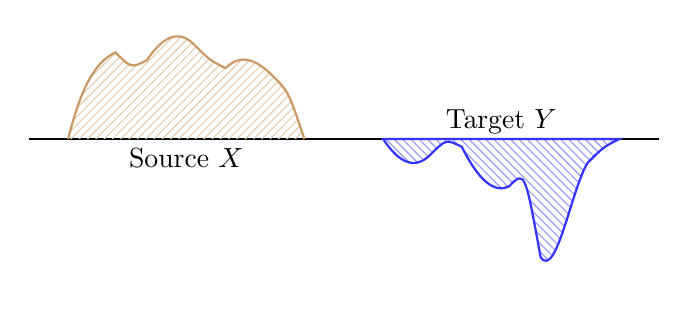
\begin{tikzpicture}[scale=1]

% Ground line
\draw[thick] (-4,-0.5) -- (4,-0.5);

% More complex pile of mass (source distribution μ) - multi-peaked
\fill[brown!60, pattern=north east lines, pattern color=brown!40] 
    (-3.5,-0.5) .. controls (-3.3,0.3) and (-3.1,0.5) .. (-2.9,0.6) 
    .. controls (-2.7,0.4) .. (-2.5,0.5) 
    .. controls (-2.3,0.8) and (-2.1,0.9) .. (-1.9,0.7)
    .. controls (-1.7,0.5) .. (-1.5,0.4)
    .. controls (-1.3,0.6) and (-1.1,0.5) .. (-0.9,0.3)
    .. controls (-0.7,0.1) .. (-0.5,-0.5) -- cycle;

\draw[thick, brown!80] 
    (-3.5,-0.5) .. controls (-3.3,0.3) and (-3.1,0.5) .. (-2.9,0.6) 
    .. controls (-2.7,0.4) .. (-2.5,0.5) 
    .. controls (-2.3,0.8) and (-2.1,0.9) .. (-1.9,0.7)
    .. controls (-1.7,0.5) .. (-1.5,0.4)
    .. controls (-1.3,0.6) and (-1.1,0.5) .. (-0.9,0.3)
    .. controls (-0.7,0.1) .. (-0.5,-0.5);

% More complex hole (target distribution ν) - multi-depression with same total area
\fill[blue!60, pattern=north west lines, pattern color = blue!40] 
    (0.5,-0.5) .. controls (0.7,-0.8) and (0.9,-0.9) .. (1.1,-0.7)
    .. controls (1.3,-0.5) .. (1.5,-0.6)
    .. controls (1.7,-1.0) and (1.9,-1.2) .. (2.1,-1.1)
    .. controls (2.3,-0.9) .. (2.5,-2.0)
    .. controls (2.7,-2.3) and (2.9,-1.1) .. (3.1,-0.8)
    .. controls (3.3,-0.6) .. (3.5,-0.5) -- cycle;

\draw[thick, blue!80] 
    (0.5,-0.5) .. controls (0.7,-0.8) and (0.9,-0.9) .. (1.1,-0.7)
    .. controls (1.3,-0.5) .. (1.5,-0.6)
    .. controls (1.7,-1.0) and (1.9,-1.2) .. (2.1,-1.1)
    .. controls (2.3,-0.9) .. (2.5,-2.0)
    .. controls (2.7,-2.3) and (2.9,-1.1) .. (3.1,-0.8)
    .. controls (3.3,-0.6) .. (3.5,-0.5) -- cycle;

% Labels
\node[below] at (-2,-0.5) {Source $X$};
\node[below] at (2,0) {Target $Y$};

\end{tikzpicture}
\end{center}
\noindent
Clearly we need that $X$ and $Y$ have the same mass and we can assume their mass is one. We can assign mass distributions $\mu$ and $\nu$ representing the mass of elements in $X$ and $Y$ respectively. Since $X$ and $Y$ both have unit mass, $\mu$ and $\nu$ are probability distributions. We need a way to determine how expensive moving some mass is, so suppose we have a function $c(x,y)$ that tells us what the cost is of transporting a unit mass from $x \in X$ to $y \in Y$. We can describe our transport plan with a function $\gamma (x,y)$, which gives how much ``mass'' it takes to move $x$ to $y$. We must have the following: 

\begin{enumerate}
    \item The amount we move out of $x$ is the same as the amount it started with. That is, \[
    \int_Y \gamma (x,y) dy = \mu (x)
    \]
    \item The amount moved into point $y$ must equal the depth of the hole. That is, \[
    \int_X \gamma (x,y) dx = \nu (y)
    \]
\end{enumerate}

% Imagine we have a distribution of mass $\mu (x)$ on space $X$ and we want to transport this mass into distribution $\nu (x)$ on the same space. 
\noindent
The total mass moved out of an infinitesimal region around $x$ must be $\mu (x) dx$, and moved into $y$ must be $\nu (y) dy$. 
Applying this to the above ideas we get \[
\int _Y \int _X \gamma (x,y) dydx = \int_X \mu (x) dx = \int_Y \nu (y) dy
\]
This is equivalent to the requirement that $\gamma$ is a joint probability distribution with marginals $\mu$ and $\nu$. The total cost of a transport plan $\gamma$ is \[
\int _Y \int _X c(x,y) \gamma (x,y) dxdy
\]
The plan $\gamma$ is not unique, and we want the optimal transport plan to be the one with the minimum total cost. We will also consider measures instead of probability distributions to account for any distribution. Any probability measure with marginals $\mu$ and $\nu$ represents a viable transport plan.

    \begin{figure}[h]
        \begin{center}
        \includegraphics[scale = 0.4]{transport.png}

        \caption{Two one dimensional distributions $\mu$ and $\nu$ and a possible joint distribution with marginals $\mu$ and $\nu$. [Credit: Wikipedia]}
\end{center}
    \end{figure}

\section{Mathematical Foundations: Optimal Transport Theory}

\subsection{Optimal Transport: The Kantorovich Problem}

Let \( (X,d_X) \) and $(Y,d_Y)$ be Polish spaces (a complete separable metric space), $(X, \mathcal{F}_1)$, $(Y, \mathcal{F}_2)$ measurable spaces, and \( \mathcal{P}(X) \) be the space of probability measures on $(X, \mathcal{F}_1)$ (similarly $\mathcal{P}(Y)$ for $(Y, \mathcal{F}_2)$). $\mathcal{P}(X \times Y)$ will denote all measures on the measurable space $(X \times Y, \mathcal{F}_1 \otimes \mathcal{F}_2)$. Let $\mu \in \mathcal{P}(X)$ and $\nu \in \mathcal{P}(Y)$:

\begin{definition}[Transport Plans]
The set of transport plans between \( \mu \) and \( \nu \) is:
\[
\Pi(\mu,\nu) = \{\gamma \in \mathcal{P}(X \times Y) : \forall A_i \in \mathcal{F}_i, \gamma (A_1 \times Y) = \mu (A_1), \gamma (X \times A_2) = \nu (A_2)\}
\]
\end{definition}
\noindent 
This is also the set of all couplings of $\mu$ and $\nu$. We can also define the set of transport plans (or couplings) in terms of pushforward measures.

\begin{definition}[Pushforward Measure]
Let $(X, \mathcal{A}_1, \upsilon)$ be a measure space, $(Y, \mathcal{A}_2)$ a measurable space, and $T : X \to Y$ be any $\mathcal{A}_1$-$\mathcal{A}_2$ measurable map. The \emph{pushforward} of $\upsilon$ under $T$, denoted $T_\# \upsilon$, is the measure on $Y$ defined by
\[
T_\# \upsilon(B) := \upsilon\big(T^{-1}(B)\big), \quad \forall B \in \mathcal{A}_2.
\]
We have that for non-negative measurable function $f : Y \to [0, \infty]$, one can show that
\[
\int_Y f(y) \, d(T_\# \upsilon)(y) = \int_X f(T(x)) \, d\upsilon(x).
\]
and this property is useful when analysing specific couplings. The fact that ${T_{\#}}{\upsilon}$ is a measure follows easily from $\upsilon$ being a measure, and preimages preserve unions.
\end{definition}

\noindent To define the set of couplings in terms of pushforward measures, define the canonical projections 
\[\pi_1: X \times Y \to X, \quad \pi_1 (x,y) = x
\]
\[
\pi_2: X \times Y \to Y, \quad \pi_2 (x,y) = y
\]
Both are clearly measurable. Then \[
{\pi _1}_{\#}\gamma (B) = \gamma (\pi_1 ^{-1} (B)) = \gamma (B \times X), \quad \forall B \in \mathcal{F}_1
\]
But since $\mu$ is the marginal of $\gamma$, we want this to be equal to $\mu (B)$. We can do a similar argument with $\nu$ and our condition in terms of pushforward measures is:
\[
\Pi(\mu,\nu) = \{\gamma \in \mathcal{P}(X \times Y) : {\pi_1}_{\#}\gamma = \mu, {\pi_2}_{\#}\gamma = \nu\}
\]
\noindent
The Kantorovich optimal transport problem seeks to minimize transportation cost over all possible transport plans, for some fixed cost function. For this, we define a cost function as any map $c: X \times Y \to [0, \infty]$ that is $\mathcal{F}_1 \otimes \mathcal{F}_2$-measurable.

\begin{definition}[Kantorovich Problem]
For a cost function \( c: X \times Y \to [0,\infty] \), the Kantorovich Formulation of the Optimal Transport problem is to find $\gamma$ attaining the infimum:
\[
\mathcal{K}(\mu,\nu) = \inf_{\gamma \in \Pi(\mu,\nu)} \int_{X \times Y} c(x,y) d\gamma(x,y)
\]
\end{definition}

\section{Mathematical Foundations: The Wasserstein Distance}

\subsection{The Wasserstein Distance}
Let $p \ge 1$ and $(X,d)$ be a Polish space. The $p$-Wasserstein distance is a special case of the Kantorovich problem when setting cost function \[
c(x,y) = d(x,y)^p
\]
and our measure space is $(X, \mathcal{B}(X))$ (the Borel $\sigma$-algebra). In this case, since the distance function is continuous, it is measurable. It is positive so it is a valid cost function. Our couplings are thus on $\mathcal{P}(X \times X)$ (i.e., we only have one metric space and consider the Kantorovich problem on that metric space)
~\\~\\ In order to define our Wasserstein metric, our space of measures is the set of measures that have finite $p$-th moments. 
\begin{definition}[Finite $p$-th Moments]
Fix $x_0 \in X$. A measure $\mu \in \mathcal{P}(X)$ is said to have finite $p$-th moment if \[
\int _X d(x,x_0)^p d\mu (x) < \infty
\]
We will denote the space of all such measures by $\mathcal{P}_p (X)$
\end{definition}

\begin{lemma}
    The choice of the reference point $x_0 \in X$ in the definition of the finite $p$-th moment does not matter. 
\end{lemma}

\begin{proof}
Suppose that for $x_0 \in X$ we have \[
    \int _X d(x, x_0)^p d\mu (x) < \infty
    \]
    Take any $x_1 \in X$. The map $x \mapsto x^p$ is convex on $[0, \infty)$ (since $p \ge 1$, its second derivative is positive), and by convexity, \[
    (d(x, x_0)+d(x_0, x_1))^p \le \frac{1}{2} (2 d(x, x_0))^p + \frac{1}{2} (2 d(x_0, x_1))^p = \frac{1}{2^{p-1}} d(x, x_0)^p + \frac{1}{2^{p-1}} d(x_0, x_1)^p
    \]which means\[
    \int _X d(x, x_1)^p d\mu (x) \le \int _X (d(x, x_0) + d(x_0, x_1))^p  d\mu (x)\le \frac{1}{2^{p-1}} \left (d(x_0, x_1)^p + \int _X d(x, x_0) d\mu (x) \right ) < \infty
    \]
\end{proof}

\begin{remark}
If we are in Euclidean space $(\mathbb{R}^n, d_E)$, a measure has finite $p$-th moment if \[
\int _{\mathbb{R}^n} |\mathbf{x}|^p d \mu (\mathbf{x}) < \infty
\]
(taking our reference point as $\mathbf{0}$)
\end{remark}

\begin{definition}[$p$-Wasserstein Distance]
Let $p \ge 1$ and consider measures \( \mu, \nu \in \mathcal{P}_p(X) \), the \( p \)-Wasserstein distance is:
\[
W_p(\mu,\nu) = \left(\inf_{\gamma \in \Pi(\mu,\nu)} \int_{X \times X} d(x,y)^p d\gamma(x,y)\right)^{1/p}
\]
We then define \[
W_\infty (\mu, \nu) := \lim \limits _{p \to \infty} W_p (\mu, \nu)
\]
\end{definition}
\noindent One can show that in this space, the lower bound $\mathcal{K}(\mu, \nu)$ is obtained.
\newpage



\begin{theorem}[Existence of an Optimal Transport Plan]
Let $\mu, \nu \in \mathcal{P}_p(X)$. Then there exists an optimal plan $\gamma^*\in\Pi(\mu,\nu)$ attaining the infimum:
\[
\mathcal{K}(\mu,\nu)
\;=\;
\int_{X\times X} d(x,y)^p\,\mathrm{d}\gamma^*(x,y).
\]
(Proved in Cédric Villani, Optimal Transport: Old and New (2009))
\end{theorem}
\noindent
The most commonly used variants of the Wasserstein metric are:
\begin{itemize}
\item \( W_1 \): The 1-Wasserstein distance, also known as the Earth Mover's Distance. This tries to minimise the total effort which is directly propertional to mass and distance 
\item \( W_2 \): The 2-Wasserstein distance. This is proportional to $\sqrt{\text{mass} \times \text{distance}^2}$ and penalises large movements more.
\item \( W_\infty \): The infinity Wasserstein distance. This represents the worst-case transport distance (the farthest any mass particle moves). Mass does not matter, only the maximum distance.
\end{itemize}
\[
\begin{array}{c|c|c|c}
\text{Metric} & \text{Meaning} & \text{Scales with mass} & \text{Scales with distance} \\ \hline
W_1 & \text{Average (mean) distance} & \times c & \times a \\
W_2 & \text{Root-mean-square distance} & \times \sqrt{c} & \times a \\
W_p & \text{\(p\)-mean distance} & \times c^{1/p} & \times a \\
W_\infty & \text{Maximum (worst-case) distance} & \text{Invariant} & \times a \\
\end{array}
\]
Consider $W_p(c\mu, c\nu)$ for $c>0$ (scaling the measures, which are no longer probabilities, but using the same formula). Then $\gamma \in \Pi(\mu,\nu) \iff c\gamma \in \Pi(c\mu,c\nu)$, scaling the total cost by $c^{1/p}$, which tends to $0$ as $p \to \infty$. Scaling distances by $a$ scales $d(x,y)^p$ by $a^p$, so the $p$th root scales the Wasserstein distance by $a$. Hence, moving mass farther becomes costlier, so for larger $p$, the optimal plan favours shorter moves. There are two key properties of the Wasserstein distance (in Villani (2009)):

\begin{theorem}[Wasserstein Distance]
For any \( p \geq 1 \), \( W_p \) defines a metric on \( \mathcal{P}_p(X) \)
\end{theorem}

% \begin{proof}
% Let $\mu, \nu, \upsilon  \in \mathcal{P}_p(X)$
% \begin{enumerate}
%     \item \textbf{Positivity: } Since our distance function is non-negative, $W_p(\mu, \nu) \ge 0$ is trivial.
%     \item \textbf{Definiteness: } First note that for measure $\mu$, consider transportation plan $\gamma (A \times B) = \mu (A \cap B)$. Define the diagonal map $\delta: X \to X \times X$ by $\delta(x) = (x,x)$ and diagonal $\Delta = \{(x,y) \in X \times X: x= y \}$. Then $\delta ^{-1} (A \times B) = A \cap B$. But then $\gamma (A \times B) = \mu (\delta ^{-1} (A \times B))$. $\mu \circ \delta^{-1}$ defines a measure. Rectangles form a 
% $\pi$-system generating the product $\sigma$-algebra; since $\gamma$ and $\mu \circ \delta ^{-1}$ are finite measures that agree on that $\pi$-system, they agree on the full $\sigma$-algebra (by the $\pi$-$\lambda$ theorem). So $\gamma = \mu \circ \gamma ^{-1}$ and thus $\gamma (\Delta) = \mu (\gamma ^{-1}(\Delta)) = \mu (X) = 1$
%     But then \[
%     \int _{X \times X} d(x,y)^p d \gamma (x,y) = \int _\Delta d(x,y)^p d\gamma(x,y) = \int_X d(\delta(x))^p d\mu (x) = \int _X \underbrace{d(x,x)^p}_{=0} d \mu (x) = 0
%     \]
%     So $W_p (\mu, \mu) = 0$. Now suppose $W_p (\mu, \nu) = 0$. Then there exists a sequence of transportation plans $(\gamma _n)_{n \in \mathbb{N}}$ such that \[
%     \int _{X \times X} d(x,y)^p d \gamma _n (x,y) \to 0 \text{ as } n \to \infty
%     \]
%     Fix a bounded $K$-Lipschitz function $\varphi : X \to \mathbb{R}$. For each $n \in \mathbb{N}$, \[
%     \left | \int _X \varphi d\mu - \int _X \varphi d \nu\ \right | = \left | \int _{X \to X} (\varphi (x) - \varphi (y)) d \gamma_n (x,y)\right | \le K \int _{X \times X} d(x,y) d \gamma _n(x,y)
%     \]
%     But then by Jensen's Inequality, \[
%     \int_{X \times X} d(x,y) d \gamma _n (x,y) \le \left (\int _{X \times X} d(x,y)^p d \gamma _n (x,y)\right) ^{1/p} \to 0
%     \]

%     But then by Theorem~\ref{thm:fortet-mourier}, we get $\mu = \nu$
%     \item \textbf{Symmetry:} For any transport plan $\gamma \in \Pi (\mu, \nu)$, define $\tilde{\gamma} (A \times B) = \gamma (B \times A)$ and then $\tilde{\gamma} \in \Pi (\nu, \mu)$ and \[
%     \int _{X \times X} d(x,y)^p d \gamma(x,y) = \int _{X \times X} d(x,y)^p d \tilde{\gamma}(x,y)
%     \]
%     So $W_p (\mu, \nu) = W_p (\nu, \mu)$
%     \item \textbf{Triangle Inequality:} See [TO ADD] for the proof.
% \end{enumerate}
% \end{proof}

\begin{theorem}[Wasserstein Completeness]
If our original metric space $(X,d)$ is complete, then the Wasserstein metric space $(\mathcal{P}_p, W_p)$ is complete
\end{theorem}

% \begin{proof} $ $
% \begin{enumerate}
% \item \textbf{Non-negativity:} For any transport plan $\gamma \in \Pi (\mu, \nu)$, since $d(x,y) \ge 0$ for all $x,y \in X$, it follows \[
% \int _{X \times X} d(x,y)^p d \gamma (x,y) \ge 0
% \]and so $W_p(\mu, \nu) \ge 0$
% \item \textbf{Vanishing property: } Suppose $W_p (\mu, \nu) = 0$. Then, for any $\varepsilon > 0$, there is a transport plan $\gamma _\varepsilon \in \Pi (\mu, \nu)$ such that \[
% \int_{X \times X} d(x,y)^p d\gamma_\varepsilon (x,y) < \varepsilon
% \]
% \item \textbf{Symmetry:} \( W_p(\mu,\nu) = W_p(\nu,\mu) \)
% \item \textbf{Triangle inequality:} \( W_p(\mu,\rho) \leq W_p(\mu,\nu) + W_p(\nu,\rho) \)
% \end{enumerate}
% \end{proof}

\section{The Kantorovich-Rubinstein Duality}

One of the most important results in optimal transport theory is the Kantorovich-Rubinstein duality theorem, which provides an equivalent characterization of the 1-Wasserstein distance. To do so, recall, for $K \ge 0$, a map $f:X \to Y$ is $K$-Lipschitz if for all $x,y \in X$, \[
d_Y(f(x), f(y)) \le K d_X(x,y)
\]

\begin{theorem}[Kantorovich-Rubinstein Duality]
For measures \( \mu, \nu \in \mathcal{P}_1(X) \) on a complete separable metric space \( (X,d) \):
\[
W_1(\mu,\nu) = \sup\left\{\int_X f d\mu - \int_X f d\nu : f: X \to \mathbb{R} \text{ is 1-Lipschitz}\right\}
\]
where we consider Lipschitz maps between $(X,d)$ and the Euclidean space $(\mathbb{R}, d_E)$.
\end{theorem}
\noindent
This duality allows us to check Lipschitz maps, instead of all possible couplings.

\begin{example}
Suppose we have measures $\mu = \frac{1}{2}(\delta _a + \delta_b)$ and $\nu = \delta _c$ for $a,b,c \in \mathbb{R}$. We expect $W_1 (\mu , \nu) = \frac{1}{2}|b-c| + \frac{1}{2}|a-c|$, as we are moving the half-mass $b$ a distance $|b-c|$ to $c$, and the same from $a$ to $c$. In this example, we are working on the space $(\mathbb{R}, d_E)$. Let $f: \mathbb{R} \to \mathbb{R}$ be $1$-Lipschitz. Then \[
\left |\int _\mathbb{R} f d\mu - \int _\mathbb{R} f d \nu \right |= \left|\frac{f(a) + f(b)}{2} - f(c) \right| = \left | \frac{f(a) - f(c)}{2} + \frac{f(b) - f(c)}{2}\right | \le \frac{1}{2} |a-c| + \frac{1}{2} | b - c|
\]
So $W_1 (\mu, \nu) \le \frac{1}{2}|a-c| + \frac{1}{2}|b-c|$. 
Without loss of generality we may assume $a \le b$. Consider cases:
\begin{enumerate}
    \item $b \le c$: Then the map $f(x) = -x$ is $1$-Lipschitz and \[
 \int _\mathbb{R} f d\mu - \int _\mathbb{R} f d\nu  = -\frac{a + b}{2} + c   = \frac{1}{2} [(c-a) + (c-b)] = \frac{1}{2} | a - c| + \frac{1}{2} |b-c|
\] 
    \item Similarly, if $c \le a$, then the map $f(x) = x$ is $1$-Lipschitz and attains the max.
    \item So suppose $a < c < b$. Define a new map $g$ as a piecewise map, with 
    \[
    g(x) = 
    \begin{cases}
        c-a & \text{ if }x \le a \\ 
        -x + c & \text{ if } a < x \le c \\ 
        x - c & \text{ if } c < x \le b \\
        b-c & \text{ if } x > b
    \end{cases}
    \]
    This is clearly $1$-Lipschitz, as each piecewise map has gradient at most 1. So \[
    \int_\mathbb{R} f d\mu - \int_\mathbb{R} f d\nu =  \frac{f(a) - f(c)}{2} + \frac{f(b) - f(c)}{2}  = \frac{c-a}{2} + \frac{b-c}{2} = \frac{1}{2} |c-a| + \frac{1}{2}|b-c|
    \]
\end{enumerate}
In every case, there is a $1$-Lipschitz map attaining the maximum which proves this example.

\end{example}

% \section{Brenier's Theorem and Optimal Maps}

% While the Kantorovich formulation allows for general transport plans, under certain conditions, optimal transport is achieved by a deterministic map. This fundamental result is known as Brenier's theorem.

% \begin{theorem}[Brenier's Theorem]
% Let \( \mu, \nu \) be probability measures on \( \mathbb{R}^d \) with \( \mu \) absolutely continuous with respect to the Lebesgue measure. Then for the quadratic cost \( c(x,y) = |x-y|^2 \), there exists a unique optimal transport plan \( \gamma^* \), and this plan is induced by a transport map \( T: \mathbb{R}^d \to \mathbb{R}^d \), i.e., \( \gamma^* = (\text{Id}, T)_\sharp\mu \).

% Moreover, \( T \) is the gradient of a convex function: \( T = \nabla \phi \) for some convex function \( \phi: \mathbb{R}^d \to \mathbb{R} \).
% \end{theorem}

% This theorem is remarkable because it establishes a deep connection between optimal transport and convex analysis. The convex function \( \phi \) is called the Kantorovich potential, and its gradient provides the optimal transportation map.

\section{Real Probability Measures}

In one dimension, the Wasserstein distance has a particularly elegant form. Consider measures \( \mu \) and \( \nu \) on \( \mathbb{R} \) with CDFs \( F \) and \( G \), respectively, where, since we are working with measures, the interpretation is that these are the CDFs of the canonical random variable $X(\omega) = \omega$. So \begin{align*}F(x) &= \mu ((-\infty, x]) \\ G(x) &= \nu ((-\infty, x])\end{align*}
We will use notation $X_\mu$ to be the canonical random variable in measure space $(\mathbb{R}, \mathcal{B}(\mathbb{R}), \mu)$. We first define the Quantile Function in terms of these CDFs:

\begin{definition}[Quantile Function]
Let \(F\colon\mathbb{R}\to[0,1]\) be a cumulative distribution function.  The \emph{quantile function} \(F^{-1}\colon[0,1]\to \overline{\mathbb{R}}\) is defined by
\[
  F^{-1}(p) = \begin{cases}\inf\{x \in \mathbb{R} : F_X(x) > 0\} & \text{if } p = 0 \\ \inf\{x \in \mathbb{R} : F_X(x) \geq p\} & \text{if } p \in (0,1]\end{cases}
\]
\end{definition}
\noindent Notice that the quantile functions are the inverse of the CDF when the CDF is bijective, possibly by restricting $F$ to its support.
Then one can show that the Wasserstein Distance is related to these quantile functions.
\begin{theorem}[One-Dimensional Wasserstein] \label{thm:1d} For $\mu, \nu \in \mathcal{P}_p(\mathbb{R})$,
\[
W_p(\mu,\nu) = \left(\int_0^1 |F^{-1}(t) - G^{-1}(t)|^p dt\right)^{1/p}
\]
where \( F^{-1} \) and \( G^{-1} \) are the quantile functions of $\mu$ and $\nu$ respectively.
\end{theorem}
\noindent
Intuitively, this is saying that our minimum transportation plan corresponds to moving the infinitesimal mass in $\mu$, corresponding to quantile $t$ in $F$ into the corresponding quantile value in $\nu$.

\begin{example}[Uniform Distributions]
Consider measure space $(\mathbb{R}, \mathcal{B}(\mathbb{R}))$ and measures $\mu, \nu \in \mathcal{P}(\mathbb{R})$ defined by \begin{align*}
\mu (A) & := \lambda _1 (A \cap [0,1]) \\ 
\nu (A) & := \frac{\lambda _1 (A \cap [0,2]) }{2}
\end{align*}
For our canonical random variable $X_\mu \sim U(0,1)$ and $X_\nu \sim U(0,2)$. Then \[F(t) = tI_{[0,1)} + I_{[1,\infty]} \Longrightarrow F^{-1}(t) = t\]
\[G(t) = \frac{1}{2}tI_{[0,2)} + I_{[2,\infty]} \Longrightarrow G^{-1}(t) = 2t\]
Both clearly have finite 1 and 2-moments, so the 1-Wasserstein and 2-Wasserstein distances are:

\[
W_1(\mu,\nu) = \int_0^1 |t - 2t| dt = \int_0^1 t dt = \frac{1}{2}
\]
\[
W_2(\mu,\nu) = \left(\int_0^1 |t - 2t|^2 dt\right)^{1/2} = \left(\int_0^1 t^2 dt\right)^{1/2} = \frac{1}{\sqrt{3}}
\]
Graphically, our optimal transport plan sends every point $x$ in $[0,1]$ into $2x$. Again, this is matching the quantiles between these distributions.
~\\
\begin{center}
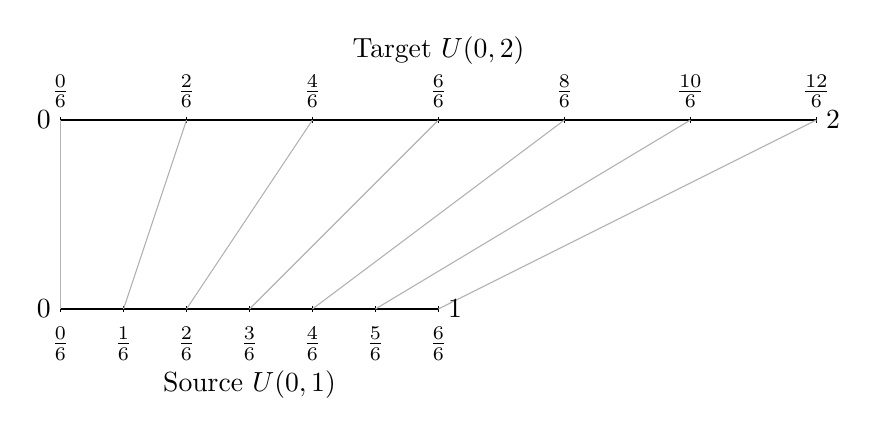
\begin{tikzpicture}[scale=0.8]
  % Draw source interval [0,1]
  \draw[line width=1pt] (0,0) -- (6,0);
  \foreach \x in {0,1,2,3,4,5,6}{
    \draw (\x,0.05) -- (\x,-0.05) node[below,yshift=-2pt] {\(\tfrac{\x}{6}\)};
  }
  \node at (3,-1.2) {Source \(U(0,1)\)};

  % Draw target interval [0,2]
  \draw[line width=1pt] (0,3) -- (12,3);
  \foreach \x in {0,2,4,6,8,10,12}{
    \draw (\x,3.05) -- (\x,2.95) node[above,yshift=2pt] {\(\tfrac{\x}{6}\)};
  }
  \node at (6,4.1) {Target \(U(0,2)\)};

  % Draw transport lines x -> 2x
  \foreach \i in {0,1,...,6}{
    \draw[gray!60] (\i,0) -- (2*\i,3);
  }

  % Annotations
  \node[left] at (0,0) {\(0\)};
  \node[right] at (6,0) {\(1\)};
  \node[left] at (0,3) {\(0\)};
  \node[right] at (12,3) {\(2\)};
\end{tikzpicture}
\end{center}

\end{example}

\section{Multivariate Normal Distributions}

For multivariate normal distributions, the Wasserstein distance has closed-form expressions that are particularly useful in applications.

\begin{theorem}[2-Wasserstein Distance Between Multivariate Normals] \label{thm:2d}
Let \( \mu = \mathcal{N}(\mathbf{m}_1, \Sigma_1) \) and \( \nu = \mathcal{N}(\mathbf{m}_2, \Sigma_2) \) be measures on \( \mathbb{R}^d \) corresponding to Multivariate Normal Distributions. Then:
\[
W_2^2(\mu,\nu) = |\mathbf{m}_1 - \mathbf{m}_2|^2 + \text{tr}(\Sigma_1 + \Sigma_2 - 2(\Sigma_1^{1/2}\Sigma_2\Sigma_1^{1/2})^{1/2})
\]
\end{theorem}

\begin{example}[Univariate Normal Distributions]
For \( \mu = \mathcal{N}(m_1, \sigma_1^2) \) and \( \nu = \mathcal{N}(m_2, \sigma_2^2) \), by Theorem~\ref{thm:2d}
\[
W_2(\mu,\nu) = \sqrt{(m_1-m_2)^2 + (\sigma_1-\sigma_2)^2}
\]
We will use Theorem~\ref{thm:1d} to find the 1-Wasserstein distance (where the CDF of a normal distribution is invertible). To do so, note that $X_ \mu \sim N(m_1, \sigma_1 ^2)$ implies $X_\mu = m_1 + \sigma_1 Z$ for $Z \sim N(0,1)$. A simple calculation shows $F(x) = \Phi \left ( \frac{x - m_1}{\sigma_1} \right)$, and so if $F^{-1}(p) = a$, then $F(a) = p$ which implies $\Phi \left (\frac{a - m_1}{\sigma_1} \right) = p$ so $\Phi ^{-1}(p) = \frac{a - m_1}{\sigma_1}$. So we have that \[
F^{-1}(p) = m_1 + \sigma_1 \Phi^{-1}(p)
\]
Thus, doing the same with $X_\nu$, \[
\int _0 ^1 |F^{-1} (p) - G^{-1}(p)|dp = \int _0 ^1 |(m_1 - m_2) + (\sigma_1 - \sigma_2) \Phi ^{-1}(p)| dp 
\]
Let $z = \Phi ^{-1}(p)$. Then our integral becomes \[
\int _{-\infty}^{\infty} |(m_1 - m_2) + (\sigma_1 - \sigma_2)z| \phi (z)dz
\]
This has a solution, and it is: \[
\begin{cases}
|m_1 - m_2|, & \text{if } \sigma_1 = \sigma_2, \\[10pt]
|m_1 - m_2|
\left[
2\,\Phi\!\left(
\dfrac{|m_1 - m_2|}{|\sigma_1 - \sigma_2|}
\right)
- 1
\right]
+ 
|\sigma_1 - \sigma_2|
\sqrt{\dfrac{2}{\pi}}
\exp\!\left(
-\dfrac{(m_1 - m_2)^2}{2(\sigma_1 - \sigma_2)^2}
\right),
& \text{if } \sigma_1 \neq \sigma_2,
\end{cases}
\]
So when the variances are the same, the 1-Wasserstein and 2-Wasserstein distances are simply the distances between the means (as we are then simply shifting a mass $1$ a total of $|m_1 - m_2|$ distance)
\end{example}

\section{Stability of the Wasserstein Distance}

The Wasserstein distances have excellent stability properties, one of which involves weak convergence.

\begin{definition}
We say a sequence of measures $(\mu_n)_{n \in \mathbb{N}}$ converges weakly to a measure $\mu$ (denoted $\mu_n \rightharpoonup \mu$) if $X_n \sim \mu_n$ and $X \sim \mu$ implies $X_n \xrightarrow{\mathcal{D}} X$
\end{definition}
\begin{theorem}[Stability Under Weak Convergence]
  Let a sequence $(\mu_n)_{n \in \mathbb{N}}\subseteq\mathcal{P}_p(X)$ and $\mu\in\mathcal{P}_p(X)$. Then the following are equivalent for :
\begin{enumerate}
  \item $W_p(\mu_n,\mu)\to0$ as $n\to\infty$.
  \item 
    \begin{enumerate}
      \item $\mu_n$ converges weakly to $\mu$ (i.e.\ $\mu_n \rightharpoonup \mu$),
      \item the $p$th moments converge. For any fixed $x_0 \in X$:
      \[
        \int_{X} d(x,x_0)^p\,d\mu_n(x)
        \to 
        \int_{X} d(x,x_0)^p\,d\mu(x)
        \quad\text{ as } n \to \infty.
      \]
    \end{enumerate}
\end{enumerate}
\end{theorem}

\noindent We can use this property to show convergence under the Wasserstein metric. 
\begin{example}
Let $\mu _n = N \left (0, \frac{1}{n} \right)$ and $\mu = \delta _0$. Let $X_n \sim \mu _n$ and $X \sim \mu$. Levy's continuity tells us that $X_n \xrightarrow{\mathcal{D}} X \iff \varphi _{X_n} \to \varphi _X$. We know that \[
\varphi_{X_n}(t) = e^{-\frac{1}{2} \frac{1}{n}t^2} \to 1 \text{ as } n \to \infty
\]
Finally, \[
\varphi _X (t) = \mathbb{E} (e^{itX}) = \int _{\mathbb{R}} e^{itX} d \delta_0 = 1
\]
So $\mu _n \rightharpoonup \mu$. Finally, \[
\int_\mathbb{R} |x|^p d\mu _n (x) = \int _{-\infty} ^{\infty} |x|^p \sqrt{\frac{{n}}{{2\pi}}} e^{-\frac{nx^2}{2}} dx = \sqrt{\frac{n}{2\pi}} 2 \int _0 ^{\infty}x^p e^{-\frac{nx^2}{2}}dx
\]
Let $u = \frac{nx^2}{2}$. Then our integral becomes \[
\sqrt{\frac{n}{2 \pi}} 2 \int _0 ^\infty \left ( \frac{2u}{n} \right)^{p/2} e^{-u} \frac{1}{\sqrt{2nu}} du = n^{-p/2} 2^{p/2} \pi ^{-1/2} \int _0 ^\infty u^{(p-1)/2} e^{-u}du = n^{-p/2} 2^{p/2} \pi ^{-1/2} \Gamma ((p+1)/2)
\]
But $p \ge 1$ implies that our integral converges to $0$ as $n \to \infty$. Finally,
\[
\int_\mathbb{R} |x|^p d \mu = 0
\]
So $\mathcal{W}_p (\mu _n, \mu) \to 0$ as $n \to \infty$
\end{example}


\section{1-Wasserstein Distances of Known Distributions}

\begin{table}[htbp]
\centering
\begin{tabular}{lll}
\hline
\textbf{Distribution} & \textbf{Parameters} & \(\displaystyle W_{1}\bigl(P_{\theta_{1}},P_{\theta_{2}}\bigr)\) \\ 
\hline
Dirac (point mass) & \(\delta_{x_{1}},\,\delta_{x_{2}}\) &
\(\lvert x_{1}-x_{2}\rvert\) \\[1ex]

Bernoulli & \(\mathrm{Bern}(p_{1}),\,\mathrm{Bern}(p_{2})\) &
\(\lvert p_{1}-p_{2}\rvert\) \\[1ex]

Uniform & \(\mathrm{Unif}(a_{1},b_{1}),\,\mathrm{Unif}(a_{2},b_{2})\) &
\(\displaystyle \int_{0}^{1} \bigl\lvert (a_{1}-a_{2})
+ t\bigl((b_{1}-a_{1})-(b_{2}-a_{2})\bigr) \bigr\rvert\, dt\) \\[2ex]

Exponential & \(\mathrm{Exp}(\lambda_{1}),\,\mathrm{Exp}(\lambda_{2})\) &
\(\displaystyle \Bigl\lvert\dfrac{1}{\lambda_{1}}-\dfrac{1}{\lambda_{2}}\Bigr\rvert\) \\[1ex]

Normal & \(\mathcal{N}(\mu_{1},\sigma_{1}^{2}),\,\mathcal{N}(\mu_{2},\sigma_{2}^{2})\) &
See Example 6.2 \\[1ex]

Gamma (fixed shape \(k\)) & \(\Gamma(k,\theta_{1}),\,\Gamma(k,\theta_{2})\) &
\(k\,\lvert\theta_{1}-\theta_{2}\rvert\) \\[1ex]
\hline
\end{tabular}
\label{tab:wasserstein1_univariate}
\end{table}
\section{A Brief Application in Colour Transfer}
We conclude with a practical application in colour transfer, where the goal is to recolour a source image to match the colour distribution of a target image while preserving structure. Representing each image as a discrete probability measure on $\mathbb{R}^3$ (where each pixel's RGB values define a point with some mass), with $\mu_S$ and $\mu_T$ denoting the source and target distributions respectively, the Wasserstein distance $W_2(\mu_S, \mu_T)$ measures the minimal cost of transforming the source distribution $\mu_S$ into the target distribution $\mu_T$. Computing the optimal transport map $T$ via computational algorithms provides a colour mapping that minimizes this cost. Applying $T$ to each source pixel produces the recoloured image. Consider the images below, with the source image (left) and target image (right), along with their colour distributions:
\begin{figure}[h]
\begin{center}
  \includegraphics[scale = 0.3]{colour_distributions.png}
\end{center}
\end{figure}
\noindent~\\
Our output image, that takes the colours in the target image and applies them to our source image, looks something like:

\begin{figure}[h]
\begin{center}
  \includegraphics[scale = 0.3]{output.png}
\end{center}
\end{figure}

\section{Conclusion}

The Optimal Transport Problem seeks the most cost-efficient transformation of one probability distribution into another. Applied to Polish spaces, this yields the Wasserstein distance, which quantifies this transformation cost between measures with finite $p$-th moments, with larger $p$ penalizing longer transport distances. The Kantorovich-Rubinstein duality characterizes the 1-Wasserstein distance via 1-Lipschitz functions, offering computational advantages. For real probability measures, $W_p$ can be computed using quantile functions, while multivariate normal distributions admit closed-form expressions. The Wasserstein metric is stable under weak convergence, making it valuable for statistical applications. These theoretical results enable diverse real-world applications wherever probability distributions arise, such as colour transfer in images and statistical inference.

\begin{thebibliography}{99}

  \bibitem{villani2009}
  C. Villani. \textit{Optimal Transport: Old and New}. Grundlehren der Mathematischen Wissenschaften, vol. 338. Springer-Verlag, Berlin, 2009.

  \bibitem{kantorovich-rubinstein1958}
  L. V. Kantorovich and G. Sh. Rubinstein. On a space of completely additive functions. \textit{Vestnik Leningrad University}, 13(7):52--59, 1958.

  \bibitem{dudley2002}
  R. M. Dudley. \textit{Real Analysis and Probability}. Cambridge University Press, Cambridge, 2002.

  \bibitem{pollard2002}
  D. Pollard. \textit{A User's Guide to Measure Theoretic Probability}. Cambridge University Press, Cambridge, 2002.

  \bibitem{ca-matran1989}
  J. A. Cuesta-Albertos and C. Matrán. Notes on the Wasserstein metric in Hilbert spaces. \textit{Annals of Probability}, 17(3):1264--1276, 1989.

  \bibitem{olkin-pukelsheim1982}
  I. Olkin and F. Pukelsheim. The distance between two random vectors with given dispersion matrices. \textit{Linear Algebra and Its Applications}, 48:257--263, 1982.

  \bibitem{billingsley1999}
  P. Billingsley. \textit{Convergence of Probability Measures}, 2nd edition. Wiley, New York, 1999.

  \bibitem{panaretos-zemel2019}
  V. M. Panaretos and Y. Zemel. Statistical aspects of Wasserstein distances. \textit{Annual Review of Statistics and Its Application}, 6:405--431, 2019.

  \bibitem{monge1781}
  G. Monge. Mémoire sur la théorie des déblais et des remblais. \textit{Histoire de l'Académie Royale des Sciences de Paris}, 1781.

  \bibitem{kantorovich1942}
  L. Kantorovich. On the translocation of masses. \textit{C.R. (Doklady) Acad. Sci. URSS (N.S.)}, 37:199--201, 1942.
\end{thebibliography}

\end{document}